We show the viability of the microservices approach in Kvik by describing the
MIxT web application for exploring and comparing transcriptional profiles from
blood and tumor samples. We also evaluate the performance of the microservices
in Kvik to show its usefulness in building MIxT. 

\subsection*{Analysis Tasks}

The web application provides functionality to perform six data analysis tasks
(A1-A6):

\textbf{A1:} Explore co-expression gene sets in tumor and blood tissue. 
We
simplify the process of exploring the computed co-expression gene sets, or
modules, through the web-application. The application
visualize gene expression patterns together with clinicopathological variables
for each module. In addition we enable users to study the underlying
biological functions of each module by including gene set analyses between the
module genes and known gene sets. 

\textbf{A2:} Explore co-expression relationships between genes. Users can
explore the co-expression relationship as a graph visualization. The network
visualizes each gene as a node and a significant co-expression relationship as
an edge.  

\textbf{A3:} Explore relationships between modules from each tissue. Users can
explore the relationship between modules from different tissues. We
provide two different metrics to compare modules, and the web application
enables users to interactively browse these relationships. In addition to
providing visualizations the compare modules from each tissue, users 
can explore the relationships, but for different breast cancer patient
groups. 

\textbf{A4:} Explore relationships between clinical variables and modules. In
addition to comparing the association between modules from both tissues, users
also have the possibility to explore the association with a module and a
specific clinical variable. It is also possible to explore the associations
stratifying on breast cancer patient group.

\textbf{A5:} Explore association between user-submitted gene lists and computed
modules. We want to enable users to explore their own gene lists to explore
them in context of the co-expression gene sets. The web application must handle
uploads of gene lists and compute association between the genelist and the MIxT
modules on demand. 

\textbf{A6:} Search for genes or gene lists of interest. To facilitate faster lookup
of genes and biological processes, the web application provides a search
functionality that lets users locate genes or gene lists and show association to
the co-expression gene sets. 


\subsection*{Design and Implementation} 
From these six analysis tasks we designed and implemented MIxT as a web
application that integrates statistical analyses and information from biological
databases together with interactive visualizations.
The MIxT web application
consists of three services: i) the web application itself containing the
user-interface and visualizations; ii) the compute service performing the MIxT
analyses delivering data to the web application; and iii) the database service
providing up-to-date information from biological databases. Each of these
services run within Docker containers making the process of deploying the
application simple. 

We structured the MIxT application with a separate view for each analysis task.
To explore the co-expression gene sets (\textbf{A1}) we built a view that
combines both static visualizations from R together with interactive tables with
gene overlap analyses. Figure \ref{fig_first_case} shows the web page presented
to users when they access the co-expression gene set 'darkturquoise' from blood.
Using the Kvik compute service we can generate plots on demand and provide users
with high-resolution PDFs or PNG files. 
% LAB: Jeg greier ikke å mappe denne informasjonen til operasjonene som er
% beksrevet ovenfor. Kanskje en figur vil hjelpe?
To explore the co-expression relationship between genes (\textbf{A2}) we use an
interactive graph visualization build with Sigmajs\footnote{\url{sigmajs.org}}.
We have built visualization for both tissues, with graph sizes of 2705 nodes and
90 348 edges for the blood network, and 2066 nodes and 50 563 edges for the
biopsy network. The sigmajs visualization library has functionality for
generating a layout for large networks, but we generate this layout server-side
to reduce the computational load on the client. To generate this layout we use
the GGally package\footnote{\url{cran.r-project.org/web/packages/GGally}}. By
generating the network layout using the compute service we relieve the clients.

% LAB: Kan også flyttes høyere opp. Hyggelig å begynne å lese noe som er lett å
% skjønne :)
To visualize relationships between modules from different tissues (\textbf{A3}), or their
relationship to clinical variables (\textbf{A4}) we built a heatmap
visualization using the d3\footnote{\url{d3js.org}} library. Figure
\ref{fig_second_case} shows an example of this heatmap visualization, showing
the association between the clinical variables and the modules from biopsy for
all samples.  

\begin{figure}[h!]
\centering
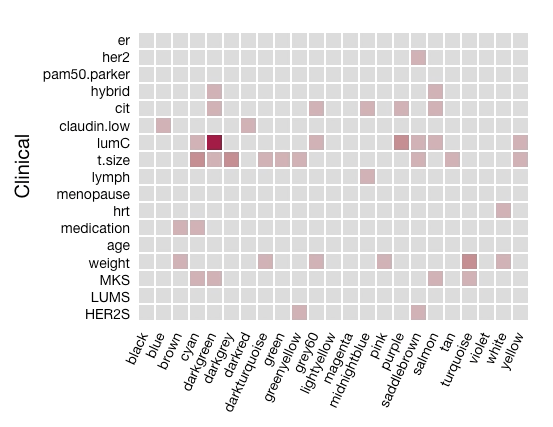
\includegraphics[width=2.5in]{figures/clinical-comp.png}
\caption{Heatmap visualization of the association between clinical variables and
the modules in biosy.  The visualization is built using the d3 JavaScript
library. The visualization can be viewed online at
\url{mixt-blood-tumor.bci.mcgill.ca/clinical-comparison}} 
\label{fig_second_case}
\end{figure} 


\begin{figure*}[h!]
\centering
\includegraphics[width=0.8\textwidth]{figures/module-3.png}
\caption{MIxT module overview page. The screenshot show the user interface for
exploring a single module. It consists of three panels. The top left panel
contains the gene expression heatmap. The top right panel contains a table of
the genes found in the module. The bottom panel contains the results of gene
overlap analyses from the module genes and known gene sets from MSigDB. The
visualization is online at
\url{mixt-blood-tumor.bci.mcgill.ca/modules/blood/darkturquoise/cohort/all}}
\label{fig_first_case}
\end{figure*} 

Since we interface directly with R we can run analyses on demand. We built a
simple upload page where users can upload their gene sets or type them in
manually (\textbf{A5}). The file is uploaded to the web application which
redirects it to the compute service that runs the analyses. Similarly we can
take user input to search for genes and processes (\textbf{A5}).


\subsection*{Evaluation} 
To investigate if it is feasible to implement parts of an application as
separate services, we evaluate the response times for a set of queries. We have
also investigated the time the MIxT web application use to produce the
visualizations for the analysis tasks. 

To evaluate the database service we measure the query time for retrieving
information about a specific gene with and without caching. This illustrates how
we can improve performance in an application by using a database service rather
than accessing the database directly.  We evaluate the query time for 1, 2, 5,
10, and 15 concurrent requests. Since the database service is just a lightweight
HTTP server we use a AWS EC2 \emph{t2.micro}\footnote{See
\url{aws.amazon.com/ec2/instance-types} for more information about AWS EC2
instance types.} instance to host it.

From the results in Table \ref{db} we see a significant improvement in response
time when the database service caches the results from the database lookups. In
addition by serving the results out of cache we reduce the number of queries to
the online database down to one. 


\begin{table}[h]
    \begin{tabular}{| l | c | c | c | c | c | }
        \hline 
        & 1 & 2 & 5 & 10 & 15 \\ 
      \hline			
      No cache & 956ms & 1123ms & 1499ms & 2147ms & 2958ms\\
      \hline
      Cache & 64ms & 64ms & 130ms & 137ms & 154ms\\
      \hline  
    \end{tabular}
    \caption[]{Time to retrieve a gene summary for a single gene, comparing
    different number of concurrent requests.}
\label{db}
\end{table} 


We evaluate the compute service by running a small microbenchmark. The benchmark
consists of two operations: first generate a set of numbers, then plot them and
return the resulting visualization. We show that the latency is low enough to
use it in an interactive application, and compare our solution to the OpenCPU
system. To show that it performs well under heavy load
we perform the same operations using 1, 2, 5, 10, and 15 concurrent requests.
We use two \emph{c4.large} instances on AWS EC2 running the Kvik
compute service and OpenCPU base docker containers. The servers have caching
disabled. 

With single requests the the mean execution time in Kvik is 274ms while OpenCPU
uses 500ms. We then investigate how each service handles concurrent requests.
Table \ref{kvikopencpucomparison} shows the time to complete the benchmark for
different number of concurrent connections. We see that the compute service in
Kvik performs better than the OpenCPU alternative. 

\begin{table}[h]
    \begin{tabular}{| l | c | c | c | c | c | }
        \hline 
       & 1 & 2 & 5 & 10 & 15 \\ 
      \hline			
      Kvik & 274ms & 278ms & 352ms & 374ms & 390ms\\
      \hline
      OpenCPU & 500ms & 635ms & 984ms & 1876ms & 2700ms\\
      \hline  
    \end{tabular}
\caption[]{Time to complete the R microbenchmark with different number of
    concurrent 
connections.}
\label{kvikopencpucomparison}
\end{table} 

We also investigate the performance of the  MIxT web application to discover
potential areas of improvement. We measured the time from an user clicks on a
link to open a specific view, until the user can interact with the results.
Table \ref{mixt-table} show the results from our evaluation, with anlysis tasks
A1 and A2 being the most time consuming. A1 generates the view in
Figure \ref{fig_first_case} which contains large HTML tables with results from
the gene set tests that take the major fraction of the time to completion. The
time to completion in analysis task A2 comes from retrieving and rendering the
two large graphs. 

\begin{table}[h]
    \resizebox{8cm}{!}{
    \begin{tabular}{  | c | c | c | c | c | c }
        \hline 
        Analysis task & Number of calls & Time to completion \\
      \hline			
      A1   & 10 &  10 seconds   \\
      A2   & 5  &  30 seconds   \\
      A3   & 1    &  2 seconds    \\
      A4   & 1   &  2 seconds   \\
      A5   &  2   &  3 seconds   \\
      A6   &  NA   &  NA  \\
      \hline  
    \end{tabular}}
\caption[]{An overview of the number of calls to the compute service and
completion time before the results for the different analysis tasks are ready to
be explored. The number of calls and completion time for analysis task 6 depends
on the search query.}
\label{mixt-table}
\end{table} 

% A2
% getalltissues,  gettomgraphnodes x2, gettomgraphedges x2
% over 15 mb of data (large networks) 

% A1
% heatmap, genelist, enrichmentschoers, goterms, bloodnormal heatmap,
% boxplot, modules x2, tissues x2
% gene set analyses, large tables 

% Kvik
% 1: 0.274
% 2: 0.278
% 5: 0.352
% 10: 0.374
% 15: 0.390 

% OPenCPU
% 1: 0.500
% 2: 0.635
% 5: 0.984
% 10: 1.876
% 15: 2.700


